\pdfminorversion=4
\documentclass[aspectratio=169]{beamer}
\usepackage{verbatim}
\newenvironment{metaverbatim}{\verbatim}{\endverbatim}
\usepackage{courier}
\usepackage{lmodern}
\usepackage{apacite}
\usepackage[hidelinks]{hyperref}
\usepackage{xcolor}
\xdefinecolor{azulcesafuerte}{HTML}{14387e}
\xdefinecolor{azulcesaclaro}{HTML}{7ab6e0}
\xdefinecolor{azulcesamedio}{HTML}{0A72BC}

\usetheme{Madrid}
%\usecolortheme[named=black]{structure}
%
\setbeamercolor{normal text}{fg=azulcesafuerte}
\setbeamercolor{background canvas}{bg=white}
\setbeamercolor{frametitle}{fg=white, bg=azulcesafuerte}
\setbeamercolor{block title}{bg=azulcesafuerte,fg=azulcesaclaro}
\setbeamercolor{navigation symbols}{}

\setbeamertemplate{background}{\tikz[overlay,remember picture]\node[opacity=0.15]at (current page.center){\includegraphics[width=6.5cm]{}};}
\usepackage{tikz}
\usepackage{kantlipsum}
\setbeamercolor*{title}{fg=white, bg=azulcesafuerte}
\setbeamercolor{titlelike}{parent=structure}

\setbeamercolor*{palette primary}{bg=azulcesafuerte,fg=white}
\setbeamercolor*{palette secondary}{bg=azulcesafuerte,fg=white}
\setbeamercolor*{palette tertiary}{bg=azulcesafuerte,fg=white}

% Change base colour beamer@blendedblue (originally RGB: 0.2,0.2,0.7)
\colorlet{beamer@blendedblue}{azulcesaclaro}
\usepackage[english]{babel}
\usepackage{apacite}
\usepackage{marvosym}
\usepackage{subfig}
\usepackage{graphicx}
\usepackage[utf8x]{inputenc}
\usepackage{url}
\usepackage{hyperref}
\usepackage{times}
\usepackage{pxfonts}
\usepackage{fontenc}
%\usepackage[dvipsnames]{xcolor}
\setbeamertemplate{bibliography item}[text]
\title[Pandas Preprocessing Useful Toolbox]{Pandas Preprocessing Useful Toolbox}
% \subtitle{(Sesión 7B)}

\author[Prof. Juan C. Correa, Ph.D.]{Prof. Juan C. Correa, Ph.D.}

\institute[]{
Colegio de Estudios Superiores de Administración\\
Bogotá - Colombia\\
\color{azulcesamedio}\Email  \href{mailto:juan.correan@cesa.edu.co}{juan.correan@cesa.edu.co}
}
\pgfdeclareimage[height=0.6cm]{OL}{OL}
 \logo{\pgfuseimage{OL}}
 \setbeamertemplate{caption}[numbered]
\date[Bogotá, Agosto, 2021] % (optional)
{}

\subject{}
\begin{document}
\begin{frame}
\titlepage
\end{frame}

% \begin{frame}
% \frametitle{Agenda} 
% \tableofcontents
% \end{frame}

\begin{frame}
\begin{block}{Learning Goal}
In data analytics, most of the analyst's time goes to data pre-processing. Being successful with these tasks requires using many tools that are somehow scattered in different books and cases. This presentation aims to provide a summary of the most useful pre-processing tasks in Python Pandas.
\end{block}
\end{frame}

\section{Documentation Sources}
\begin{frame}
\begin{center}
\Huge
\textcolor{azulcesaclaro}{1\\
--------------------------------\\
Documentation Sources}
\end{center}
\end{frame}

\begin{frame}
Although the Pandas textbook was published some years ago, updated manuals have been released more recently \cite{McKinney2021}
\begin{figure}

\includegraphics[width=.2\textwidth]{pandas.jpeg}
\end{figure}
\centering
\textcolor{blue}{\url{https://pandas.pydata.org/docs/pandas.pdf}}
\end{frame}

\begin{frame}
Apart from Pandas' updated manuals, we will use the textbook of \citeauthor{Molin2021} \citeyear{Molin2021}
\begin{figure}

\includegraphics[width=.2\textwidth]{book.png}
\end{figure}
Its public repository is available at:
\centering
\textcolor{blue}{\url{https://github.com/stefmolin/Hands-On-Data-Analysis-with-Pandas-2nd-edition}}
\end{frame}

\begin{frame}
It is good to cloning the repo to follow the sintaxes explained in each chapter.
\begin{figure}
\centering
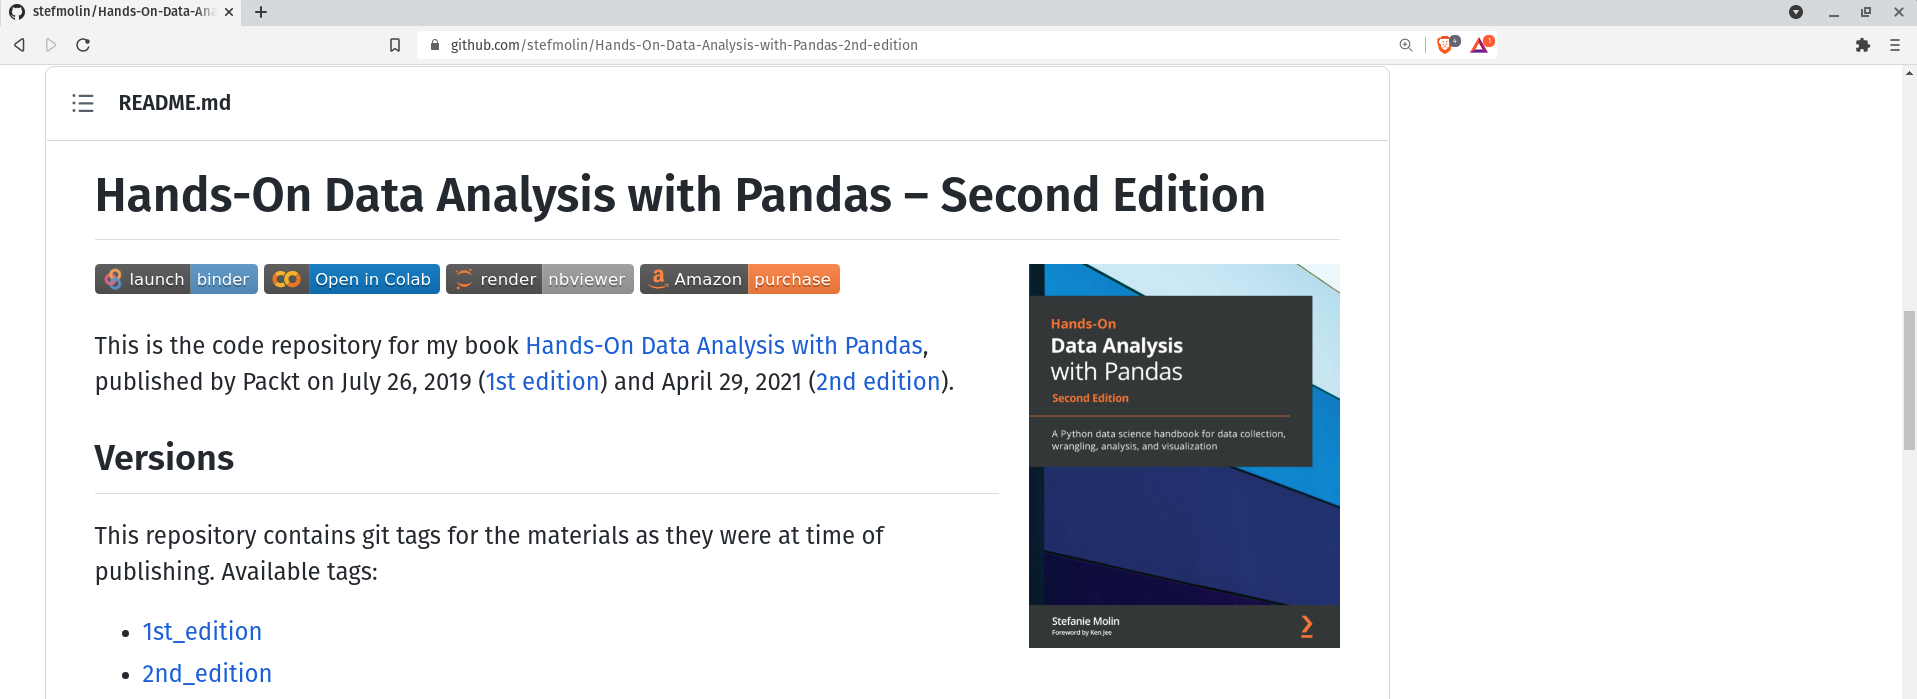
\includegraphics[width=.85\textwidth]{github1.png}
\end{figure}
\end{frame}

\section{Useful Sintaxes}
\begin{frame}
\begin{center}
\Huge
\textcolor{azulcesaclaro}{2\\
--------------------------------\\
Useful Sintaxes}
\end{center}
\end{frame}

\subsection{Indexing Operations}
\begin{frame}{Indexing Operations}
Indexing operations provide a one-method way to select both the rows and the columns of a dataframe. We can use \texttt{loc[]} and \texttt{iloc[]} to subset our dataframe using label-based or integer-based lookups, respectively. A good way to remember the difference is to think of them as location versus integer location.
\end{frame}

\begin{frame}
\begin{figure}
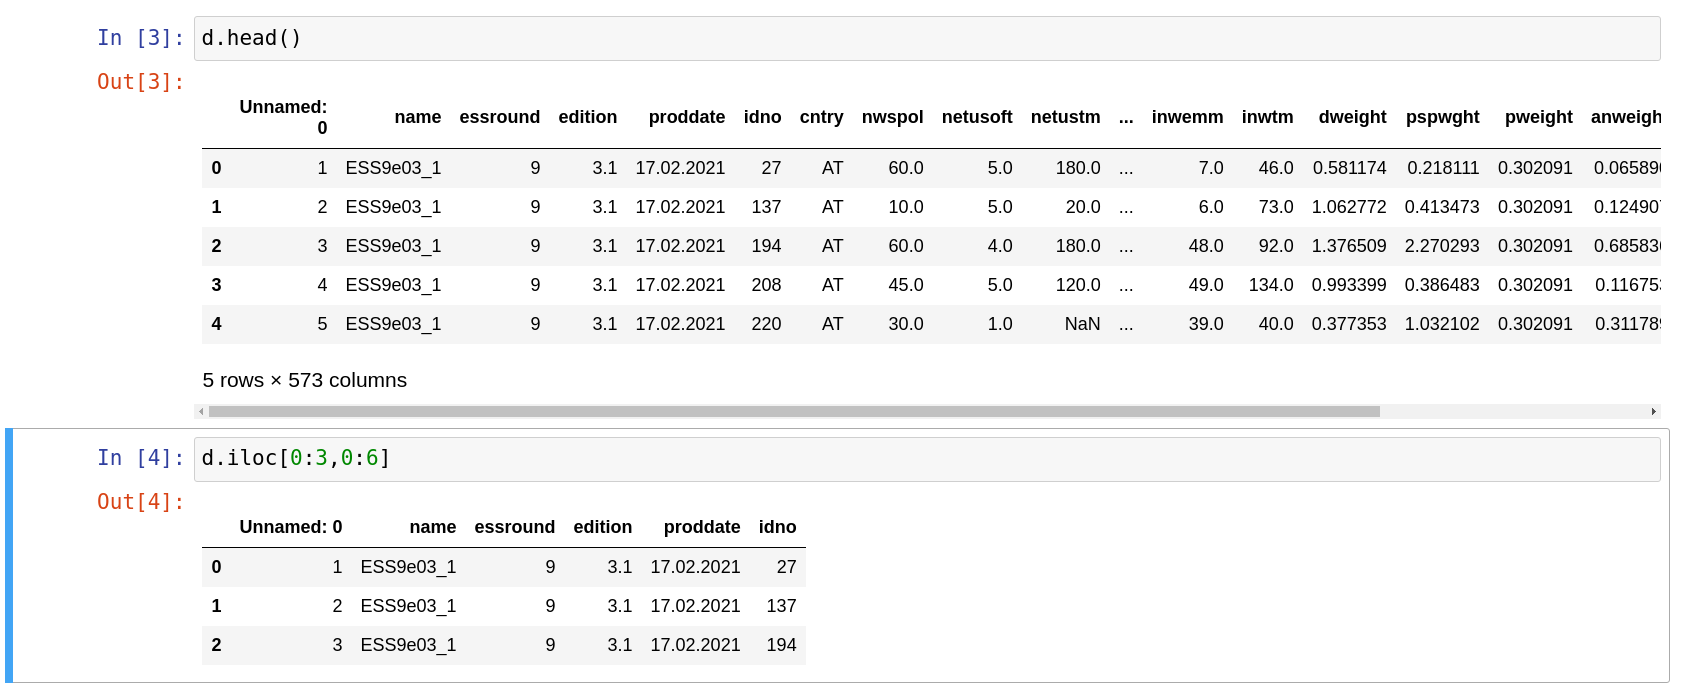
\includegraphics[width=.75\textwidth]{selecting.png}
\end{figure}
Here, the first three rows and the first six columns of the ``d'' dataframe are selected with \texttt{d.iloc[0:3,0:6]}
\end{frame}

\begin{frame}
\begin{figure}
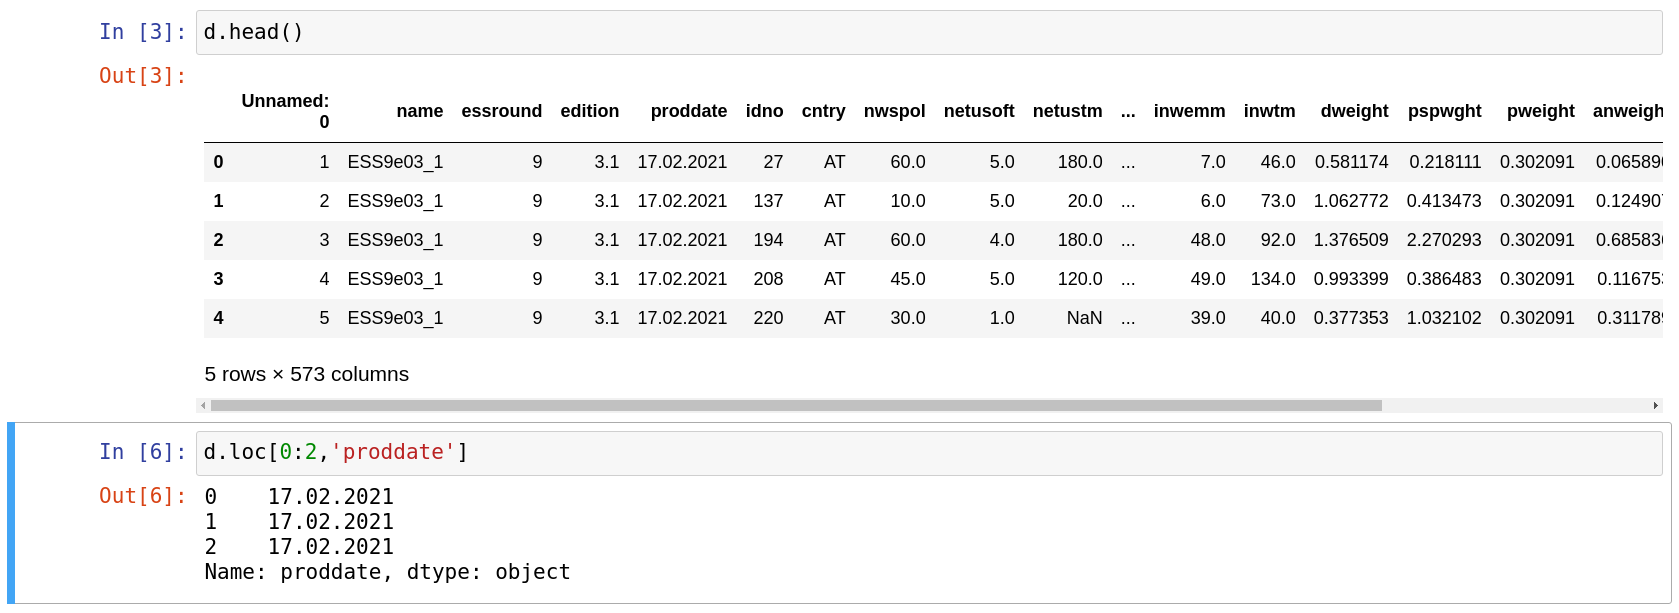
\includegraphics[width=.75\textwidth]{indexing.png}
\end{figure}
Here, in contrast, with \texttt{d.loc[0:2,'proddate']} we are subsetting the first three rows of the column \texttt{\textcolor{red}{'proddate'}}
\end{frame}

\begin{frame}[allowframebreaks]{Referencias}
\tiny{ 
\bibliographystyle{apacite}
\bibliography{REFS.bib}
} 
\end{frame}

\setbeamertemplate{background}{\tikz[overlay,remember picture]\node[opacity=1]at (current page.center){
\includegraphics[width=18cm]{ulam.png}};}
\pgfdeclareimage[height=0cm,width=0cm]{}{}
 \logo{\pgfuseimage{}}
\beamertemplatenavigationsymbolsempty
\begin{frame}
\end{frame}
\end{document}